% License: CC BY-SA
% Authors: See the authors below and see also acknowledgement for authors of some images or research

\documentclass[25pt, margin=0mm, innermargin=25mm, blockverticalspace=25mm, colspace=25mm, subcolspace=8mm]{tikzposter}
\geometry{paperwidth=63in,paperheight=42in}

% to stretch boxes over whole paper with custor paper size
\makeatletter
\setlength{\TP@visibletextwidth}{\textwidth-2\TP@innermargin}
\setlength{\TP@visibletextheight}{\textheight-2\TP@innermargin}
\makeatother

% Fira Sans, GRASS GIS branding sans serif font
\usepackage{FiraSans}
\renewcommand*\oldstylenums[1]{{\firaoldstyle #1}}

% EB Garamond, GRASS GIS branding serif font
% note that EB Garamond does not have bold
\usepackage[cmintegrals,cmbraces]{newtxmath}
\usepackage{ebgaramond-maths}

% might be needed for both font packages
\usepackage[T1]{fontenc}

% uncomment for all sans serif
% \renewcommand{\familydefault}{\sfdefault}


\usepackage[utf8]{inputenc}
\usepackage{wrapfig}
\usepackage[hidelinks]{hyperref}
\usepackage{alltt}

% For bibliography styling
%% TODO: all names should be abbreviated
\usepackage{natbib}

\definecolor{textcolor}{HTML}{000000}

\definecolor{titleTextColor}{HTML}{000000}
\definecolorpalette{grassColorPalette} {
  \definecolor{colorOne}{HTML}{419041}
  % \definecolor{colorTwo}{HTML}{cccccc}
  \definecolor{colorTwo}{HTML}{dddddd}
  \definecolor{colorThree}{HTML}{F1B52D}
  % \definecolor{colorThree}{HTML}{EFA126}
}

\usetheme{Default}
\usetitlestyle{Empty}
\usecolorstyle[colorPalette=grassColorPalette]{Britain}
\colorlet{backgroundcolor}{white}

\title{
\Huge
\textcolor{titleTextColor}{
\textsf{
% \textbf{
\fontsize{130}{100}\selectfont
\begin{minipage}{\textwidth}
\centering
Software Citation with Fine Granularity:
\\[1cm]
The \textnormal{\textsf{\textit{g.citation}}} Module for \textbf{GRASS}\,{\firalight GIS}
\end{minipage}
% }
}
}
}

\newlength{\grasslogoheight}
\setlength{\grasslogoheight}{0.09\textheight}
\newlength{\instlogoheight}
\setlength{\instlogoheight}{0.33\grasslogoheight}

% \setlength{\blocktitleheight}{0.02\textheight}

% style for institute numbers
\newcommand{\inst}[1]{\hspace{2pt}$^{\mbox{\normalsize#1}}$\hspace{-7pt}}
\newcommand{\instlist}[1]{\hspace{1pt}$^{\mbox{\normalsize#1}}$\hspace{2pt}}

\author{
Vaclav Petras\inst{1}\,*\hspace{-7pt},
Peter Loewe\inst{2},
Markus Neteler\inst{3},
\&
Helena Mitasova\inst{1}
}

\institute{
\large
\instlist{1}Center for Geospatial Analytics, North Carolina State University, USA;
\instlist{2}DIW Berlin Deutsches Institut für Wirtschaftsforschung e.V., Germany;
\instlist{3}mundialis GmbH \& Co. KG, Germany;
*Corresponding author: wenzeslaus@gmail.com, vpetras@ncsu.edu
\\[1.7cm]

\includegraphics[height=3cm]{ncstate}%
\hspace{1cm}%

\includegraphics[height=3cm]{cga}%
\hspace{2.7cm}%

\includegraphics[height=3cm]{diw_berlin}%
\hspace{3cm}%

\includegraphics[height=3.4cm]{mundialis}%
}

% \author{
%
% % Vaclav Petras\inst{1}\,*,
% % Peter Loewe\inst{2},
% % Markus Neteler\inst{3},
% % \&
% % Helena Mitasova\inst{1},
% }
% \institute{
% \large
% % \instlist{1}Center for Geospatial Analytics, North Carolina State University, USA;
% % \instlist{2}DIW Berlin Deutsches Institut für Wirtschaftsforschung e.V., Germany;
% % \instlist{3}mundialis GmbH \& Co. KG, Germany;
% *Corresponding author: wenzeslaus@gmail.com, vpetras@ncsu.edu;
% **Over 10 other members of the core team and numerous other contributors
% \\[1.7cm]
% 
\includegraphics[height=3cm]{ncstate}%
% \hspace{1cm}%
% 
\includegraphics[height=3cm]{cga}%
% \hspace{3cm}%
% 
\includegraphics[height=3.4cm]{mundialis}%
% \hspace{3cm}%
% 
\includegraphics[height=3cm]{diw_berlin}%
% }

\hypersetup
{
    pdfauthor={H. Mitasova, V. Petras, A. Petrasova, M. Neteler},
    pdfsubject={AGU Fall Meeting 2018 Poster},
    pdftitle={Software Citation with Fine Granularity: The g.citation Module for GRASS GIS},
    pdfkeywords={GIS, algorithms, methods, preservation, science, reproducibility}
}

% \usetemplate{1}
% \setinstituteshift{1}

% \setblocktitleheight{2}
% \setblockspacing{1}

\graphicspath{{images/}{logos/}}

\newcommand{\blocktitlewrap}[1]{\textnormal{\textsf{\textsc{\huge#1}}}}
% it is not possible (?) to change block title in the class, using wrapper
% the command introduced using:
%   sed -i 's/\\block{\([^}]*\)}/\\block{\\blocktitlewrap{\1}}/g' main.tex

% bullet point style
\renewcommand{\labelitemi}{\textcolor{gray}{$\bullet$}\hspace{0.5ex}}

% GRASS module
\newcommand{\gmodule}[1]{\href{http://grass.osgeo.org/grass72/manuals/#1.html}{\emph{#1}}}
\newcommand{\gamodule}[1]{\href{http://grass.osgeo.org/grass72/manuals/addons/#1.html}{\emph{#1}}}
\newcommand{\gmodulenolink}[1]{\emph{#1}}

\begin{document}

\node[above left,opacity=0.99,inner sep=0pt,outer sep=4cm] at (bottomleft -| topright)%
  {
\includegraphics[width=0.3\paperwidth]{grass}};

\maketitle[width=0.92\textwidth]

% \maketitle
% \addlogo[north west]{(2,-1)}{9cm}{images/Grass_GIS}
%Please insert your institution logo here
% \addlogo[north east]{(-2,-2.5)}{4cm}{images/logo_FEM_CRI}
% \addlogo[north east]{(-2,-5.5)}{4cm}{images/NC_State_Seal}
% \addlogo[north east]{(-8,-2.5)}{4cm}{images/Logo_cvut}
% \addlogo[north east]{(-8,-6.5)}{4cm}{images/IWMI_logo}
% \addlogo[north east]{(-2,-10.5)}{4cm}{images/logo_ec-jrc}

\begin{columns}

% Abstract
%
% GRASS GIS (grass.osgeo.org) is a community-driven geospatial software project
% with a record of being used in scientific publications and research projects
% over three decades. Authors of scientific publications, when using and citing
% GRASS GIS, so far opted for citing either the entire software package, citing
% the most recent review publication associated with GRASS GIS, or citing a
% publication associated with a specific module.
%
% GRASS GIS provides over 500 modules, each with a unique functionality and
% purpose, many with associated scientific publications. In addition to these core
% modules in the GRASS GIS distribution there is a growing number of additional
% add-on modules are being developed, often as part of research work. Until now,
% no automated, software-enabled citation mechanism to cite individual GRASS GIS
% modules, or functions in general was provided due to the lack of a reference
% citation standard for GRASS GIS modules defined within the GRASS GIS community.
%
% We present a new GRASS GIS module g.citation with the aim to provide a
% convenient, concise, and standardized way of citing GRASS GIS and its individual
% modules. The current version of g.citation extracts the relevant information
% from a respective manual page of any given GRASS GIS module and turns this
% semi-structured record into a proper citation in a variety of styles and formats
% with the machine-readable Citation File Format (CFF) currently promising most
% efficiency and expressiveness in storing the information and Citation Style
% Language (CSL) used for formatting citations. The module is now in a prototype
% stage and it is available in the GRASS GIS Addons repository. Future directions
% include using standardized format for storing the citation information together
% with the code and incorporating persistent scientific identifiers such as DOI.
% We are now seeking collaborators and feedback from authors of geospatial
% algorithms who want to share their code and be cited at the same time.

%%%%%%%%%%%%%%%%%%%%%%%%%%%%%%%%%%%%%%%%%%%%%%%%%%%%%%%%%%%%%%%%%%%%%
%%%%%%%%%%%%%%%%%%%%%%%%%%%%%%%%%%%%%%%%%%%%%%%%%%%%%%%%%%%%%%%%%%%%%
%%%%%%%%%%%%%%%%%%%%%%%%%%%%%%%%%%%%%%%%%%%%%%%%%%%%%%%%%%%%%%%%%%%%%
%%%%%%%%%%%%%%%%%%%%%%%%%%%%%%%%%%%%%%%%%%%%%%%%%%%%%%%%%%%%%%%%%%%%%
\column{0.25}

%%%%%%%%%%%%%%%%%%%%%%%%%%%%%%%%%%%%%%%%%%%%%%%%%%%%%%%%%%%%%%%%%%%%%%%%%%%%%%%
\block{\blocktitlewrap{GRASS GIS Overview}}{

\Large

\begin{itemize}
% Basic Topics
 \item Community-driven project
 \item 35 years of continuous software development
 \item long-term releases, stable APIs, and emphasis on science
 \item single integrated environment for 2D and 3D raster analysis, image processing, vector data analysis, and spatio-temporal data processing
\end{itemize}

}

%%%%%%%%%%%%%%%%%%%%%%%%%%%%%%%%%%%%%%%%%%%%%%%%%%%%%%%%%%%%%%%%%%%%%%%%%%%%%%%
\block{\blocktitlewrap{Current Approaches}}{

\Large

Authors of scientific publications, when using and citing
GRASS GIS, so far opted for citing either the entire software package, citing
the most recent review publication associated with GRASS GIS, or citing a
publication associated with a specific module.

\vspace*{1.5cm}

\begin{minipage}{\linewidth}
\centering
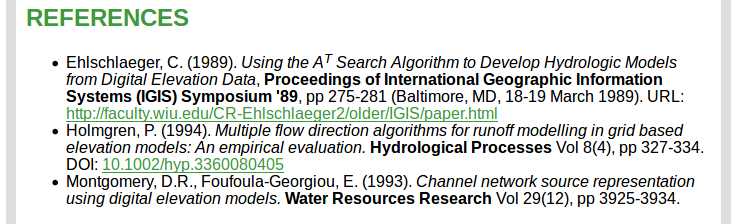
\includegraphics[width=.7\linewidth]{module_references}
\\
Creating a synchronized animation of monthly total precipitation and mean temperature for NC, USA
\end{minipage}

\vspace*{1cm}

\vspace*{1.5cm}

\begin{minipage}{\linewidth}
\centering

\includegraphics[width=.7\linewidth]{module_author}
\\
Creating a synchronized animation of monthly total precipitation and mean temperature for NC, USA
\end{minipage}

\vspace*{1cm}

}

%%%%%%%%%%%%%%%%%%%%%%%%%%%%%%%%%%%%%%%%%%%%%%%%%%%%%%%%%%%%%%%%%%%%%%%%%%%%%%%
\block{\blocktitlewrap{Motivation}}{

\Large

GRASS GIS provides over 500 modules, each with a unique functionality and
purpose, many with associated scientific publications. In addition to these core
modules in the GRASS GIS distribution there is a growing number of additional
add-on modules are being developed, often as part of research work. Until now,
no automated, software-enabled citation mechanism to cite individual GRASS GIS
modules, or functions in general was provided due to the lack of a reference
citation standard for GRASS GIS modules defined within the GRASS GIS community.

}

%%%%%%%%%%%%%%%%%%%%%%%%%%%%%%%%%%%%%%%%%%%%%%%%%%%%%%%%%%%%%%%%%%%%%
%%%%%%%%%%%%%%%%%%%%%%%%%%%%%%%%%%%%%%%%%%%%%%%%%%%%%%%%%%%%%%%%%%%%%
%%%%%%%%%%%%%%%%%%%%%%%%%%%%%%%%%%%%%%%%%%%%%%%%%%%%%%%%%%%%%%%%%%%%%
%%%%%%%%%%%%%%%%%%%%%%%%%%%%%%%%%%%%%%%%%%%%%%%%%%%%%%%%%%%%%%%%%%%%%
\column{0.25}

%%%%%%%%%%%%%%%%%%%%%%%%%%%%%%%%%%%%%%%%%%%%%%%%%%%%%%%%%%%%%%%%%%%%%%%%%%%%%%%
\block{\blocktitlewrap{GRASS GIS Documentation}}{

\Large


}

%%%%%%%%%%%%%%%%%%%%%%%%%%%%%%%%%%%%%%%%%%%%%%%%%%%%%%%%%%%%%%%%%%%%%%%%%%%%%%%
\block{\blocktitlewrap{GRASS GIS Metadata for Modules}}{

\Large


}

%%%%%%%%%%%%%%%%%%%%%%%%%%%%%%%%%%%%%%%%%%%%%%%%%%%%%%%%%%%%%%%%%%%%%%%%%%%%%%%
\block{\blocktitlewrap{\textnormal{\textsf{\textit{g.citation}}} Module}}{

\Large

\vspace*{1.5cm}

\begin{minipage}{\linewidth}
\centering
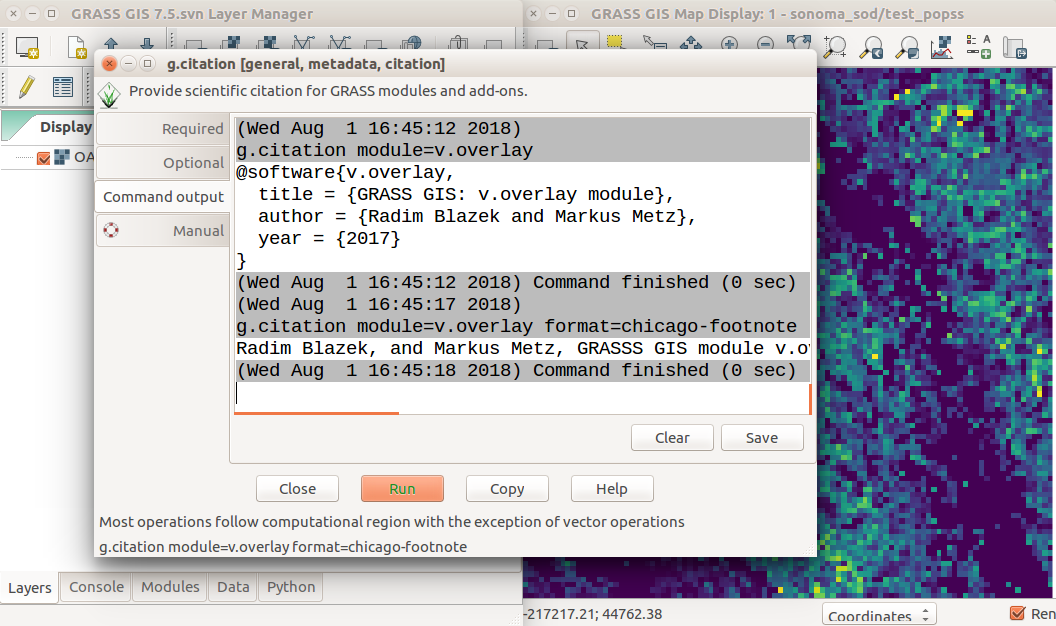
\includegraphics[width=.7\linewidth]{screenshot_bibtex_chicago}
\\
Creating a synchronized animation of monthly total precipitation and mean temperature for NC, USA
\end{minipage}

\vspace*{1cm}

}

%%%%%%%%%%%%%%%%%%%%%%%%%%%%%%%%%%%%%%%%%%%%%%%%%%%%%%%%%%%%%%%%%%%%%%%%%%%%%%%
\block{\blocktitlewrap{Citation File Format (CFF)}}{

\Large

\begin{itemize}
 \item YAML (YAML Ain’t Markup Language) text file
 \item human- and machine- readable
 \item \texttt{CITATION.cff} file
\end{itemize}

\vspace*{.5cm}

\begin{minipage}{\linewidth}
\centering
\includegraphics[width=.7\linewidth]{code/cff}
\\
Creating a synchronized animation of monthly total precipitation and mean temperature for NC, USA
\end{minipage}

\vspace*{1cm}

}

%%%%%%%%%%%%%%%%%%%%%%%%%%%%%%%%%%%%%%%%%%%%%%%%%%%%%%%%%%%%%%%%%%%%%%%%%%%%%%%
\block{\blocktitlewrap{Citation Style Language (CSL)}}{

\Large

\begin{itemize}
 \item style language for citations
 \item citeproc-py CSL processor
 \item metadata $\rightarrow$ CSL + citeproc JSON $\rightarrow$ journal citation
\end{itemize}

}

%%%%%%%%%%%%%%%%%%%%%%%%%%%%%%%%%%%%%%%%%%%%%%%%%%%%%%%%%%%%%%%%%%%%%
%%%%%%%%%%%%%%%%%%%%%%%%%%%%%%%%%%%%%%%%%%%%%%%%%%%%%%%%%%%%%%%%%%%%%
%%%%%%%%%%%%%%%%%%%%%%%%%%%%%%%%%%%%%%%%%%%%%%%%%%%%%%%%%%%%%%%%%%%%%
%%%%%%%%%%%%%%%%%%%%%%%%%%%%%%%%%%%%%%%%%%%%%%%%%%%%%%%%%%%%%%%%%%%%%
\column{0.25}

%%%%%%%%%%%%%%%%%%%%%%%%%%%%%%%%%%%%%%%%%%%%%%%%%%%%%%%%%%%%%%%%%%%%%%%%%%%%%%%
\block{\blocktitlewrap{Discussion and Future Work}}{

\Large


}


%%%%%%%%%%%%%%%%%%%%%%%%%%%%%%%%%%%%%%%%%%%%%%%%%%%%%%%%%%%%%%%%%%%%%%%%%%%%%%%%
\block{\blocktitlewrap{References}}{

\vspace{-0.2cm}
\scriptsize

% \newcommand{\blocksectiontitle}[1]{\subsubsection*{\textcolor{gray}{\textsf{#1}}}}
\newcommand{\blocksectiontitle}[1]{\textbf{#1}}

%\blocksectiontitle{References}
\begingroup
\renewcommand{\section}[2]{}%
\bibliographystyle{apalike}
% \bibliography{poster}
\endgroup

}

%%%%%%%%%%%%%%%%%%%%%%%%%%%%%%%%%%%%%%%%%%%%%%%%%%%%%%%%%%%%%%%%%%%%%
%%%%%%%%%%%%%%%%%%%%%%%%%%%%%%%%%%%%%%%%%%%%%%%%%%%%%%%%%%%%%%%%%%%%%
%%%%%%%%%%%%%%%%%%%%%%%%%%%%%%%%%%%%%%%%%%%%%%%%%%%%%%%%%%%%%%%%%%%%%
%%%%%%%%%%%%%%%%%%%%%%%%%%%%%%%%%%%%%%%%%%%%%%%%%%%%%%%%%%%%%%%%%%%%%
\column{0.25}


%%%%%%%%%%%%%%%%%%%%%%%%%%%%%%%%%%%%%%%%%%%%%%%%%%%%%%%%%%%%%%%%%%%%%%%%%%%%%%%
\block{\blocktitlewrap{Availability}}{

\Large

\begin{itemize}
 \item
 \item
 \item
 \item
\end{itemize}

}

\end{columns}

\node[above left,opacity=0.5,inner sep=0pt,outer sep=4cm] at (bottomleft -| topright)%
  {
\includegraphics[width=0.3\paperwidth]{grass}};

\end{document}
